\chapter{Valutazione Empirica}
In questo capitolo verranno discussi nel dettaglio gli esperimenti realizzati nell'ambito di questa tesi. Verranno esposte le scelte adoperate nella selezione e realizzazione degli esperimenti e nella raccolta dei risultati.\\
Infine, verranno presentati e discussi i risultati raccolti.\\\\
Nella sezione 4.1 sono descritti gli esperimenti realizzati e vengono giustificate le scelte riguardanti gli iperparametri selezionati. Nella sezione 4.2 sono infine presentati in dettaglio i risultati finali ottenuti nell'ambito di questa tesi.
\section{Esperimenti}
\subsection{Panoramica} 
Gli esperimenti sono stati eseguiti su un personal computer con sistema operativo Windows 10 in versione developer build 21390.2025 e all'interno della Windows Subsystem for Linux, con supporto alla GPU. Il computer monta una GPU nVidia GeForce GTX 1070 con 6 Gb di memoria dedicata, una CPU Intel i5 3570 e 12 Gb di RAM.\\\\
Le \textit{callback} utilizzate durante le sessioni di addestramento sono state le seguenti:
\begin{itemize}
    \item[-] \textit{TensorBoard}, per poter visualizzare in tempo reale l'andamento dell'addestramento delle varie reti.
    \lstinputlisting[style=myPython, firstnumber=61, firstline=61, lastline=61]{code/wesad_totaltrain.py}
    \item[-] \textit{EarlyStopping}, per poter fermare anticipatamente l'addestramento in caso di diverse epoche svolte senza ottenere risultati migliori. La fermata anticipata è stata impostata sulla loss calcolata sul validation set, con pazienza di 10 epoche e ripristino dei migliori pesi trovati della rete neurale.
    \lstinputlisting[style=myPython, firstnumber=60, firstline=60, lastline=60]{code/wesad_totaltrain.py}
\end{itemize}
Tutti gli esperimenti sono stati eseguiti con batch di 256 elementi e per una durata massima 100 epoche, a meno di fermata anticipata. Inoltre il training set è sempre stato diviso in 75\% training set e 25\% validation set.
\lstinputlisting[style=myPython, firstnumber=63, firstline=63, lastline=63]{code/wesad_totaltrain.py}
\subsection{Model Selection}
Il modello adoperato per ogni dataset è stato selezionato in base all'accuratezza che esso ha raggiunto durante l'addestramento offline. L'approccio alla model selection è stato il medesimo per entrambi i dataset, delineato di seguito:
\begin{enumerate}
    \item Selezione dei parametri dell'ottimizzatore\\
    L'algoritmo di ottimizzazione selezionato è Adam, poiché consigliato per problemi con molti dati rumorosi, efficiente in termini di tempo e spazio in memoria e facilità di fine-tuning degli iperparametri$^{\cite{adampaper}}$.\\
    Lo spazio dei parametri preso in considerazione è stato:
    \begin{itemize}
        \item[-] \textit{Learning rate} $\in \{0.001, 0.005, 0.008, 0.01\}$
        \item[-] $\beta_1 \in \{0.8, 0.85, 0.9, 0.95, 0.99\}$
        \item[-] $\beta_2 \in \{0.98, 0.985, 0.99, 0.995, 0.999\}$
    \end{itemize}
    \item Selezione dei parametri di regolarizzazione\\
    Il regolarizzatore L1L2 è stato applicato sul kernel, sui bias e sui valori d'uscita del layer di output.\\
    I parametri presi in considerazione sono:
    \begin{itemize}
        \item[-] Kernel $\in \{0.0001, 0.00001, 0.000001\}$
        \item[-] Bias $\in \{0.0001, 0.00001, 0.000001\}$
        \item[-] Output $\in \{0.0001, 0.00001, 0.000001\}$
    \end{itemize}
    \item Selezione della struttura della rete neurale\\
    La rete neurale è stata scelta in base al miglior risultato ottenuto dopo 5 epoche di addestranmento.\\
    Le configurazioni prese in considerazione sono:
    \begin{itemize}
        \item[-] Layer $\in \{1, 2, 3, 4\}$
        \item[-] Unità $\in [10, 40]$
    \end{itemize}
\end{enumerate}
Questo procedimento ha prodotto i seguenti modelli, uno per dataset:
\begin{itemize}
    \item[-] Dataset \textbf{WESAD}\\
    Due layer nascosti composti da 18 unità GRU con i seguenti parametri:
    \begin{itemize}
        \item[-] \textit{Learning rate} $= 0.005$
        \item[-] $\beta_1 = 0.99$
        \item[-] $\beta_2 = 0.99$
        \item[-] Kernel, bias, output $= 0.0001$
    \end{itemize}
    Il modello è capace di raggiungere in modo consistente il 99\% di accuratezza sul dataset durante l'addestramento offline. Questo lo rende un ottimo candidato per giudicare l'applicabilità dello stesso modello su diverse metodologie di continual learning.
    \item[-] Dataset \textbf{ASCERTAIN}\\
    Due layer nascosti composti da 24 unità GRU con i seguenti parametri:
    \begin{itemize}
        \item[-] \textit{Learning rate} $= 0.01$
        \item[-] $\beta_1 = 0.9$
        \item[-] $\beta_2 = 0.99$
        \item[-] Kernel, bias, output $= 0.00001$
    \end{itemize}
    Anche questo modello è stato selezionato in base all'accuratezza sul dataset, che si attesta intorno al 45\%.
\end{itemize}
La scelta dei modelli si è basata sui risultati ottenuti nell'addestramento offline poiché è interessante comparare la differenza di risultati ottenuti negli scenari dove i dati di addestramento diventano disponibili nel tempo, cioè le metodologie di Addestramento Continuo, allo scenario in cui i dati sono disponibili sin da subito. Questo consente di verificare il cambiamento di prestazioni del solito modello nei diversi casi.
\subsection{Percentuale di replay}
La percentuale di dati da ripetere nella sessione di addestramento successiva, secondo lo scenario di replay, è stata scelta provando diversi valori percentuali in base all'accuratezza e alle altre metriche misurate nell'Addestramento Continuo naive sul dataset WESAD, con i risultati presentati nella tabella \ref{tab:replayperctest}.\\
\begin{table}[h]
    \begin{center}
        \begin{tabular}{l|c|c|c|c}
            \textbf{Percentuale} & \textbf{Accuratezza} & \textbf{ACC} & \textbf{BWT} & \textbf{FWT}\\
            \hline
            $10\%$ & 74,55\% & 0,7589 & 0,007 & 0,5539\\
            $15\%$ & 75,94\% & 0,7593 & -0,005 & 0,4693\\
            $20\%$ & 74,50\% & 0,7568 & 0,0054 & 0,3342\\
            \textbf{25\%} & \textbf{74,83\%} & \textbf{0,7707} & \textbf{0,0158} & \textbf{0,5275}\\
            $33\%$ & 74,71\% & 0,7823 & 0,0105 & 0,5948\\
        \end{tabular}
        \caption{Comparazione fra diverse percentuali di replay}
        \label{tab:replayperctest}
    \end{center}
\end{table}
La scelta è ricaduta sul 25\% di replay poiché le metriche misurate sono mediamente più alte delle altre percentuali, in particolare nel trasferimento di conoscenza. Inoltre, dalle prove effettuate, l'incremento dell'accuratezza derivato dall'aumentare la percentuale di replay è risultato irrisorio. La scelta è stata ulteriormente influenzata dall'utilizzo di memoria, e un valore maggiore porta a modelli migliori pur usando più memoria durante l'addestramento.
\subsection{Numero di esempi nelle memorie episodiche}
Per quanto riguarda lo scenario episodico, l'iperparametro $m$ indica il numero di esempi per ogni classe che vengono mantenuti fra una sessione di addestramento e l'altra. Tale iperparametro è stato scelto provando diversi valori sulla base dell'accuratezza e delle altre metriche misurate nell'addestranento episodico su dataset WESAD, ottenendo i risultati elencati nella tabella \ref{tab:episodicmtest}\\\\
\begin{table}[h]
    \begin{center}
        \begin{tabular}{l|c|c|c|c}
            \textbf{$m =$} & \textbf{Accuratezza} & \textbf{ACC} & \textbf{BWT} & \textbf{FWT}\\
            \hline
            $40$ & 79,07\% & 0,8450 & 0,0516 & 0,3752\\
            $50$ & 78,08\% & 0,8082 & 0,0253 & 0,5651\\
            $60$ & 79,50\% & 0,8979 & 0,0998 & 0,6109\\
            \textbf{70} & \textbf{81,11\%} & \textbf{0,8589} & \textbf{0,0447} & \textbf{0,6351}\\
            $80$ & 80,83\% & 0,9064 & 0,0957 & 0,4223\\
            $90$ & 80,92\% & 0,9031 & 0,0892 & 0,4793
        \end{tabular}
        \caption{Comparazione fra vari valori di $m$ nell'addestramento episodico}
        \label{tab:episodicmtest}
    \end{center}
\end{table}\\
Viene scelto $m = 70$ poiché raggiunge un'accuratezza media superiore e un'accettabile trasferimento di conoscenza. Anche qua la scelta è dettata dall'utilizzo di memoria, e come dimostrato dai dati un valore maggiore di $m$ può risultare in generale preferibile.

\pagebreak
% Tabelle e grafici di ogni esperimento, con confronti fra i continual
\section{Risultati finali}
\paragraph{WESAD} Usando come modello una rete neurale con due layer nascosti composti da 18 unità GRU e un layer di output con 4 unità aventi funzione di attivazione \textit{softmax}, su WESAD sono stati ottenuti i seguenti risultati:
\begin{table}[h]
\footnotesize
    \begin{tabular}{l|c|c|c|c|c|c|c}
        \textbf{Scenario} & \textbf{Epoche} & \textbf{Tempo} & \textbf{Acc.} & \textbf{ACC} & \textbf{BWT} & \textbf{FWT} & \textbf{Memoria}\\
        \hline
        \textbf{Offline} & 28 & 94,69s & 99,07 & - & - & - & 2061,40 Mb\\
        \textbf{Continual} & 49,14$\pm$33,67 & 947,24s & 73,13$\pm$4,02 & 0,7721 & 0,0343 & 0,5397 & 2173 Mb\\
        \textbf{Cumulative} & 39,71$\pm$19,91 & 2786s & 81,97$\pm$8,67 & 0,961 & 0,1383 & 0,4674 & 2291,45 Mb\\
        \textbf{Replay} & 41,14$\pm$21,19 & 1063,51s & 78,29$\pm$3,32 & 0,7849 & -0,002 & 0,4582 & 2184,77 Mb\\
        \textbf{Episodic} & 35$\pm$26,26 & 1088,29s & 82,13$\pm$6,60 & 0,9095 & 0,0841 & 0,4226 & 2097,47 Mb\\
        \textbf{EWC} & 29,71$\pm$17,38 & 1342,81s & 70,74$\pm$4,74 & 0,7251 & 0,0113 & 0,4698 & 2187,40 Mb\\
        \textbf{LWF} & 44,29$\pm$18,30 & 3282,51s & 69,09$\pm$5,82 & 0,7419 & 0,0451 & 0,3248 & 2121,31 Mb\\
    \end{tabular}
    \caption{Risultati WESAD}
    \label{tab:reswesad}
\end{table}\\
\begin{figure}[h]
	\begin{center}
		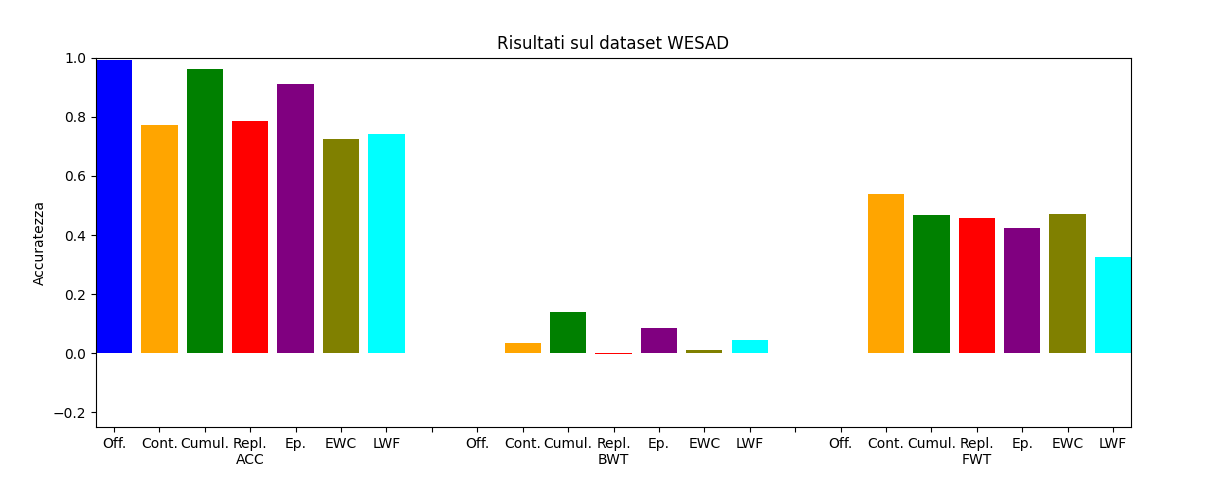
\includegraphics[width=0.95\textwidth]{img/graphs/wesad_final_metrics.png}
		\caption{Risultati su WESAD}
		\label{fig:wesad_metrics_graph}
	\end{center}
\end{figure}\\
L'accuratezza del 99\% raggiunta nel training offline dimostra come il dataset WESAD sia particolarmente adatto all'inferenza da parte di reti neurali ricorrenti dalla bassa complessità. Con poco più di 25 epoche di addestramento, abbiamo ottenuto un modello capace di classificare con un alto grado di accuratezza lo stato psico-fisico di un utente.\\
Ciò che è interessante notare è che l'accuratezza è mantenuta sopra il 70\% anche nella maggior parte delle metodologie continue. La performance peggiore media la si ha nel \textit{Learning Without Forgetting}, che però ottiene comunque un'accuratezza finale (ACC) del 74\% e un FWT comunque ottimo. La miglior performance tra le metodologie continue è ottenuta dall'apprendimento cumulativo, con un'accuratezza finale del 96\% perfettamente paragonabile alla metodologia offline, e in linea con la teoria. In tutti gli approcci, si ha un FWT elevato e molto superiore al BWT, segnale che ogni soggetto migliora molto l'apprendimento sui soggetti successivi, mentre non vi è particolare influenza sui precedenti soggetti o, se vi è, è positiva.\\\\
L'esperimento quindi dimostra come l'Apprendimento Continuo su dati sensoriali come respirazione, temperatura, elettrocardiogramma e simili possa portare a modelli con performance paragonabili all'apprendimento offline. Con un po' di \textit{fine-tuning} e \textit{model selection} con le metodologie continue si può probabilmente trovare un modello con performance ancora superiori a quelle sperimentate.
\begin{figure}[h]
	\begin{center}
		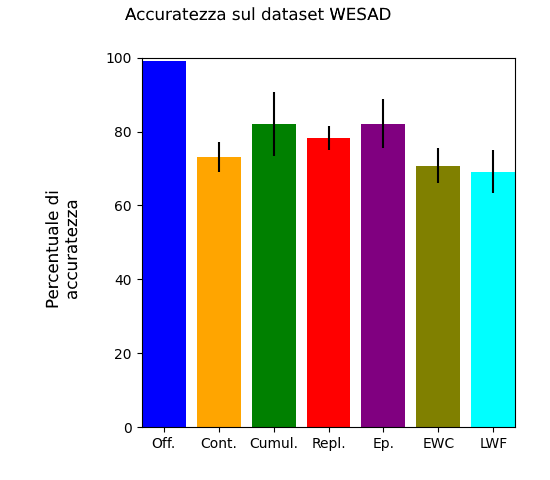
\includegraphics[width=0.65\textwidth]{img/graphs/wesad_final_accuracy.png}
		\caption{Accuratezza su WESAD}
		\label{fig:wesad_accuracy_graph}
	\end{center}
\end{figure}
\paragraph{ASCERTAIN} Usando come modello una rete neurale con due layer nascosti composti da 24 unità GRU e un layer di output con 4 unità aventi funzione di attivazione \textit{softmax}, su ASCERTAIN sono stati raggiunti i seguenti risultati:
\begin{table}[h]
\footnotesize
    \begin{tabular}{l|c|c|c|c|c|c|c}
        \textbf{Scenario} & \textbf{Epoche} & \textbf{Tempo} & \textbf{Acc.} & \textbf{ACC} & \textbf{BWT} & \textbf{FWT} & \textbf{Memoria}\\
        \hline
         \textbf{Offline} & 3 & 29,14s & 42,78 & - & - & - & 1817,28 Mb\\
        \textbf{Continual} & 10,88$\pm$5,01 & 249,28s & 37,45$\pm$5,01 & 0,25 & -0,0168 & 0,0213 & 2154,36 Mb\\
        \textbf{Cumulative} & 9,25$\pm$6,81 & 932,56s & 39,06$\pm$4,26 & 0,2697 & 0,0064 & 0,0278 & 2297,17 Mb\\
        \textbf{Replay} & 13,25$\pm$10,03 & 402,96s & 39,48$\pm$4,37 & 0,2603 & -0,014 & 0,0485 & 2173,95 Mb\\
        \textbf{Episodic} & 12,62$\pm$7,94 & 498,24s & 38,80$\pm$4,04 & 0,2742 & 0,0048 & 0,0156 & 2231,42 Mb\\
        \textbf{EWC} & 24,14$\pm$16,94 & 810,96s & 36,08$\pm$5,66 & 0,2497 & -0,0183 & -0,0003 & 2171,62 Mb\\
        \textbf{LWF} & 21,62$\pm$10,20 & 879,68s & 35,69$\pm$5,43 & 0,2448 & 0.0327 & 0,0156 & 2103 Mb\\
    \end{tabular}
    \caption{Risultati ASCERTAIN}
    \label{tab:resascertain}
\end{table}\\
\begin{figure}[h]
	\begin{center}
		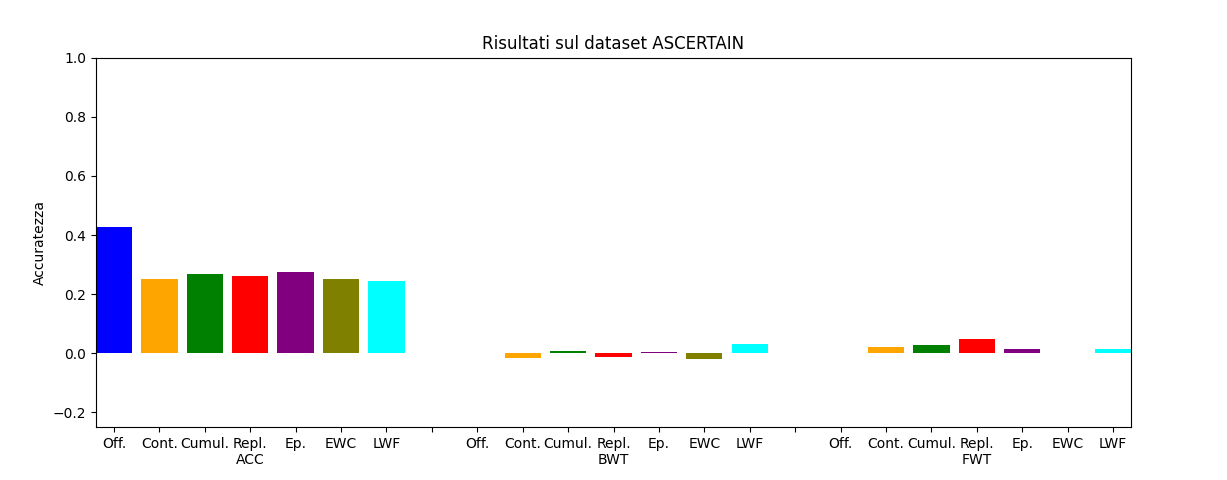
\includegraphics[width=0.95\textwidth]{img/graphs/ascertain_final_metrics.png}
		\caption{Risultati sul dataset ASCERTAIN}
		\label{fig:ascertain_metrics_graph}
	\end{center}
\end{figure}\\
Dalla metodologia offline è subito chiaro come il dataset ASCERTAIN presenti una difficoltà maggiore rispetto a WESAD. In particolare, il dataset ASCERTAIN presenta dati particolarmente sbilanciati sulla classe 0 e informazioni riguardo le espressioni facciali dei soggetti durante l'esperimento, dati di difficile classificazione.\\
Le metodologie continue sono comunque in linea con i risultati sul precedente dataset, con la performance peggiore ottenuta dal \textit{Learning Without Forgetting} mentre la migliore è ottenuta dalla metodologia cumulativa anche grazie ad un BWT superiore alla metodologia replay. In molti casi si nota un valore negativo di trasferimento di conoscenza all'indietro, sintomo di un lieve caso di \textit{catastrophic forgetting}.\\\\
Per poter dimostrare l'impatto dovuto allo sbilanciamento delle classi, il dataset ASCERTAIN è stato riorganizzato in soggetti "fittizi" come esposto di seguito.
\paragraph{Custom ASCERTAIN} Dopo aver eseguito il preprocessing specificato precedentemente, tutti i dati di addestramento sono stati uniti in un unico insieme. Da questo insieme è stato estratto il test set, e il rimanente training set è stato suddiviso in 17 soggetti bilanciati e composti da 108 sequenze di 160 punti ciascuna.\\
Usando come modello una rete neurale con due layer nascosti composti da 24 unità GRU e un layer di output con 4 unità aventi funzione di attivazione \textit{softmax}, su ASCERTAIN con i soggetti fittizi sono stati registrati i seguenti risultati:
\begin{table}[h]
\footnotesize
    \begin{tabular}{l|c|c|c|c|c|c|c}
        \textbf{Scenario} & \textbf{Epoche} & \textbf{Tempo} & \textbf{Acc.} & \textbf{ACC} & \textbf{BWT} & \textbf{FWT} & \textbf{Memoria}\\
        \hline
         \textbf{Offline} & 29 & 66,17s & 87,77 & - & - & - & 1945,91 Mb\\
        \textbf{Continual} & 7,75$\pm$5,33 & 226,24s & 87,01$\pm$0,64 & 0,2481 & -0,0241 & 0,0052 & 2143,71 Mb\\
        \textbf{Cumulative} & 7,25$\pm$8,80 & 872,8s & 87,66$\pm$0,16 & 0,2773 & 0,0032 & 0,0801 & 2273,07 Mb\\
        \textbf{Replay} & 12,125$\pm$12,94 & 299,52s & 87,13$\pm$0,75 & 0,2711 & -0,0012 & 0,306 & 2146,35 Mb\\
        \textbf{Episodic} & 5,5$\pm$3,94 & 319,76s & 82,19$\pm$3,95 & 0,339 & 0,0346 & 0,1043 & 2204,84 Mb\\
        \textbf{EWC} & 14,38$\pm$7,58 & 541,68s & 87,34$\pm$0,42 & 0,2467 & -0,0191 & 0,0845 & 2146,36 Mb\\
        \textbf{LWF} & 20,75$\pm$8,42 & 771,36s & 86,91$\pm$0,89 & 0,2495 & -0,0333 & -0,146 & 2095,93 Mb\\
    \end{tabular}
    \caption{Risultati su ASCERTAIN con soggetti fittizi bilanciati}
    \label{tab:rescustomascertain}
\end{table}\\
\begin{figure}[h]
	\begin{center}
		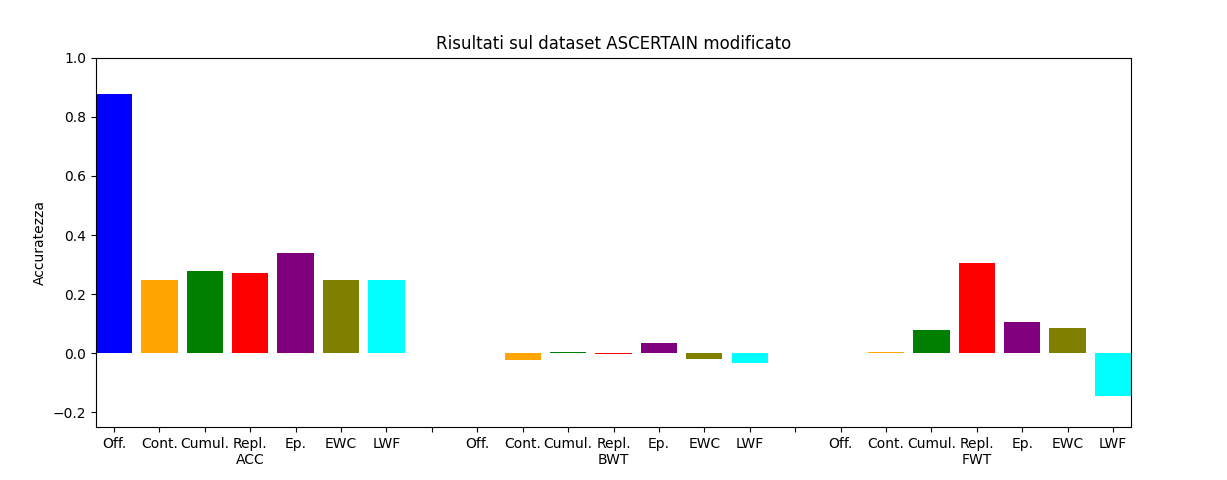
\includegraphics[width=0.95\textwidth]{img/graphs/customascertain_final_metrics.png}
		\caption{Risultati su ASCERTAIN con soggetti fittizi}
		\label{fig:customascertain_metrics_graph}
	\end{center}
\end{figure}\\
Dalla tabella \ref{tab:rescustomascertain} si evince subito come il bilanciamento abbia prodotto accuratezze medie molto superiori al dataset originale: la metodologia offline raggiunge l'87,77\% di accuratezza, paragonabile ai risultati ottenuti sul dataset WESAD, e le metodologie continue, in linea coi precedenti risultati, superano comunque l'80\% di accuratezza media in tutti i casi.\\
Dalle rimanenti metriche si nota comunque la difficoltà intrinseca del dataset, che raggiunge un'accuratezza finale del solo 33\% con la metodologia di replay episodico e BWT spesso negativo o comunque molto basso.
\begin{figure}[!tbp]
    \begin{minipage}[b]{0.5\textwidth}
		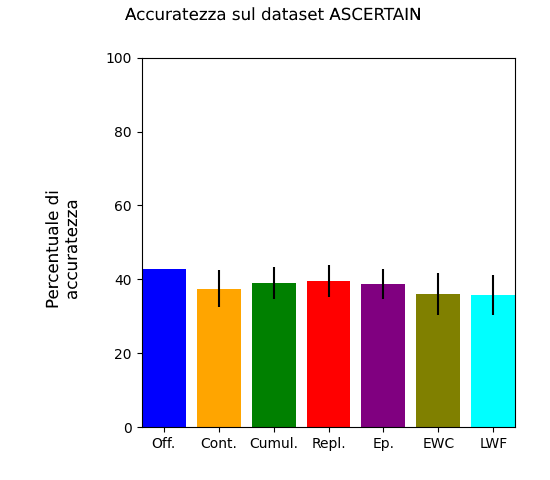
\includegraphics[width=\textwidth]{img/graphs/ascertain_final_accuracy.png}
		\caption{Accuratezza sul dataset ASCERTAIN originale}
		\label{fig:ascertain_accuracy_graph}
	\end{minipage}
    \hfill
    \begin{minipage}[b]{0.5\textwidth}
		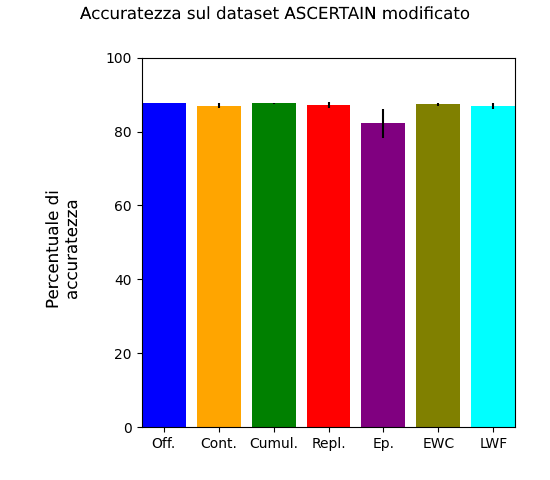
\includegraphics[width=\textwidth]{img/graphs/customascertain_final_accuracy.png}
		\caption{Accuratezza su ASCERTAIN con soggetti fittizi}
		\label{fig:customascertain_accuracy_graph}
	\end{minipage}
\end{figure}
Questa variazione del dataset ASCERTAIN dimostra come il bilanciamento dei dati di training sia fondamentale nel corretto addestramento di una rete neurale. L'avere dei soggetti di partenza bilanciati a livello di classi contenute, e di conseguenza esempi di addestramento non fortemente sbilanciati su una o più classi come nel caso del dataset ASCERTAIN originale, porta ad avere un'addestramento della rete neurale di miglior qualità e risultati finali sensibilmente migliori.
\pagebreak
\section{Metodologie Continue a Confronto}
Dai risultati ottenuti e elencati nelle tabelle \ref{tab:reswesad}, \ref{tab:resascertain} e \ref{tab:rescustomascertain} possiamo mettere a confronto fra loro le diverse metodologie di continual learning prese in considerazione.
\begin{table}[h]
\footnotesize
    \begin{tabular}{l|c|c|c|c|c|c|c}
        \textbf{Dataset} & \textbf{Epoche} & \textbf{Tempo} & \textbf{Acc.} & \textbf{ACC} & \textbf{BWT} & \textbf{FWT} & \textbf{Memoria}\\
        \hline
        \textbf{WESAD} & 49,14$\pm$33,67 & 947,24s & 73,13$\pm$4,02 & 0,7721 & 0,0343 & 0,5397 & 2173 Mb\\
        \textbf{ASCERTAIN} & 10,88$\pm$5,01 & 249,28s & 37,45$\pm$5,01 & 0,25 & -0,0168 & 0,0213 & 2154,36 Mb\\
        \textbf{Cust. ASC.} & 7,75$\pm$5,33 & 226,24s & 87,01$\pm$0,64 & 0,2481 & -0,0241 & 0,0052 & 2143,71 Mb\\
        \hline
        Media & 22,59 & 474,25s & 65,86 & 0,4234 & -0,0022 & 0,1887 & 2157,02 Mb
    \end{tabular}
    \caption{Risultati delle metodologia naive}
    \label{tab:rescontinual}
\end{table}\\
La metodologia continua più semplice ottiene sui dataset risultati sempre comparabili alla metodologia offline utilizzata come baseline. Come elencato in tabella \ref{tab:rescontinual}, la metodologia continual su dataset WESAD ottiene un'accuratezza media del 73.13\%, da confrontare con la metodologia offline con un'accuratezza del 99.07\%. Questo primo risultato porta ad una considerazione: su dataset come WESAD, contente dati ben bilanciati nelle classi, già solo la metodologia continua più triviale ottiene risultati non ottimi ma comunque buoni, anche dimostrato dalla metrica BWT di 0.0343 e dall'FWT di 0.5397 che indicano un buon trasferimento della conoscenza.\\
ASCERTAIN d'altro canto ottiene solo un risultato del 42.78\% offline, ma anche qua la metodologia continual ottiene un paragonabile 37.45\% di accuratezza media, nonostante l'accuratezza finale solo del 25\% (che su quattro classi da inferire è equivalente allo scegliere una classe in modo casuale). ASCERTAIN con i soggetti fittizi, invece, ottiene un 87.01\% di accuratezza sulla metodologia naive a fronte dell'87.77\% ottenuto dalla metodologia offline, dimostrando l'importanza delle classi bilanciate, ma ottenendo solo il 24.81\% di accuratezza finale.
\begin{table}[h]
\footnotesize
    \begin{tabular}{l|c|c|c|c|c|c|c}
        \textbf{Dataset} & \textbf{Epoche} & \textbf{Tempo} & \textbf{Acc.} & \textbf{ACC} & \textbf{BWT} & \textbf{FWT} & \textbf{Memoria}\\
        \hline
        \textbf{WESAD} & 39,71$\pm$19,91 & 2786s & 81,97$\pm$8,67 & 0,961 & 0,1383 & 0,4674 & 2291,45 Mb\\
        \textbf{ASCERTAIN} & 9,25$\pm$6,81 & 932,56s & 39,06$\pm$4,26 & 0,2697 & 0,0064 & 0,0278 & 2297,17 Mb\\
        \textbf{Cust. ASC.} & 7,25$\pm$8,80 & 872,8s & 87,66$\pm$0,16 & 0,2773 & 0,0032 & 0,0801 & 2273,07 Mb\\
        \hline
        Media & 18,74 & 1530,45s & 69,56 & 0,5027 & 0,0493 & 0,1918 & 2287,23 Mb
    \end{tabular}
    \caption{Risultati della metodologia cumulative}
    \label{tab:rescumulative}
\end{table}\\
La metodologia cumulativa, i cui risultati sono elencati nella tabella \ref{tab:rescumulative}, evidenzia fin da subito l'effetto che il replay degli esempi ha sull'addestramento continuativo.\\
Sul dataset WESAD, la metodologia cumulativa raggiunge un'accuratezza media dell'81.97\% e finale del 96.10\%, cioè quasi a livello con la metodologia offline che ottiene un'accuratezza del 99.07\%. Anche BWT e FWT evidenziano un buon trasferimento della conoscenza, attestandosi rispettivamente su 0.1383 e 0.4674.\\
Il dataset ASCERTAIN evidenzia ancora una volta la propria difficoltà, con un'accuratezza media della metodologia cumulativa pari a 39.06\% e finale del 26.97\%, comunque molto inferiore rispetto al 42.78\% dell'addestramento offline. Con i soggetti bilanciati, otteniamo un'accuratezza media dell'87.66\%, da comparare al quasi identico 87.77\% di accuratezza della metodologia offline, ma un'accuratezza finale del 27.73\%. In entrambi i casi, il BWT indica un trasferimento all'indietro della conoscenza quasi nullo, rispettivamente dello 0.0064 e dello 0.0032, e analogamente l'FWT, dello 0.0278 e dello 0.0801 rispettivamente.
\begin{table}[h]
\footnotesize
    \begin{tabular}{l|c|c|c|c|c|c|c}
        \textbf{Dataset} & \textbf{Epoche} & \textbf{Tempo} & \textbf{Acc.} & \textbf{ACC} & \textbf{BWT} & \textbf{FWT} & \textbf{Memoria}\\
        \hline
        \textbf{WESAD} & 41,14$\pm$21,19 & 1063,51s & 78,29$\pm$3,32 & 0,7849 & -0,002 & 0,4582 & 2184,77 Mb\\
        \textbf{ASCERTAIN} & 13,25$\pm$10,03 & 402,96s & 39,48$\pm$4,37 & 0,2603 & -0,014 & 0,0485 & 2173,95 Mb\\
        \textbf{Cust. ASC.} & 12,125$\pm$12,94 & 299,52s & 87,13$\pm$0,75 & 0,2711 & -0,0012 & 0,306 & 2146,35 Mb\\
        \hline
        Media & 22,17 & 588,66s & 68,30 & 0,4388 & -0,0057 & 0,2709 & 2168,36 Mb
    \end{tabular}
    \caption{Risultati della metodologia con il 25\% di replay}
    \label{tab:resreplay}
\end{table}\\
Comparandolo al 99.07\% della metodologia offline, sul dataset WESAD avere il 25\% di replay fa ottenere risultati ovviamente inferiori all'81.97\% della metodologia continuativo ma consente comunque di superare il 73.13\% della metodologia naive, ottenendo un 78.29\% di accurateza media e un 78.49\% di accuratezza finale. Nonostante il BWT di -0.002, quasi nullo, si ha un buon trasferimento in avanti della conoscenza come provato dall'FWT di 0.4582.\\
ASCERTAIN ha un comportamento simile: la metodologia che usa il il 25\% di replay ottiene il 39.48\% di accuratezza media e il 26.03\% di accuratezza finale che supera la metodologia continual e anche quella cumulativa. Lo stesso non si può dire di ASCERTAIN con i soggetti fittizi, che come per WESAD ottiene un'accuratezza sul 25\% di replay che si attesta a metà tra la metodologia continual e quella cumulativa. I risultati sono elencati nella tabella \ref{tab:resreplay}.
\begin{table}[h]
\footnotesize
    \begin{tabular}{l|c|c|c|c|c|c|c}
        \textbf{Dataset} & \textbf{Epoche} & \textbf{Tempo} & \textbf{Acc.} & \textbf{ACC} & \textbf{BWT} & \textbf{FWT} & \textbf{Memoria}\\
        \hline
        \textbf{WESAD} & 35$\pm$26,26 & 1088,29s & 82,13$\pm$6,60 & 0,9095 & 0,0841 & 0,4226 & 2097,47 Mb\\
        \textbf{ASCERTAIN} & 12,62$\pm$7,94 & 498,24s & 38,80$\pm$4,04 & 0,2742 & 0,0048 & 0,0156 & 2231,42 Mb\\
        \textbf{Cust. ASC.} & 5,5$\pm$3,94 & 319,76s & 82,19$\pm$3,95 & 0,339 & 0,0346 & 0,1043 & 2204,84 Mb\\
        \hline
        Media & 17,71 & 635,43s & 67,70 & 0,5076 & 0,0412 & 0,1808 & 2177,91 Mb
    \end{tabular}
    \caption{Risultati della metodologia episodica con $m = 70$}
    \label{tab:resepisodic}
\end{table}\\
Utilizzando un replay statico e bilanciato nelle classi, vale a dire la metodologia episodica i cui risultati sono elencati in tabella \ref{tab:resepisodic}, su WESAD otteniamo risultati comparabili alla metodologia cumulativa pur usando quasi il 10\% in meno di memoria: la metodologia episodica raggiunge l'82.13\% di accuratezza media mentre quella cumulativa l'81.97\%, ottenendo però un'accuratezza finale del 96.10\% rispetto al 90.95\% della metodologia episodica.\\
Sul dataset ASCERTAIN abbiamo una situazione simile: la metodologia cumulativa ottiene il 38.80\% di accuratezza mentre con quella episodica si raggiunge il 39.06\% usando il 3\% in meno di memoria. Lo stesso discorso non si può dire per il dataset ASCERTAIN con i soggetti fittizi, che ottiene un'accuratezza media dell'82.19\% inferiore all'87.66\% della metodologia cumulativa.
\begin{table}[h]
\footnotesize
    \begin{tabular}{l|c|c|c|c|c|c|c}
        \textbf{Dataset} & \textbf{Epoche} & \textbf{Tempo} & \textbf{Acc.} & \textbf{ACC} & \textbf{BWT} & \textbf{FWT} & \textbf{Memoria}\\
        \hline
        \textbf{WESAD} & 29,71$\pm$17,38 & 1342,81s & 70,74$\pm$4,74 & 0,7251 & 0,0113 & 0,4698 & 2187,40 Mb\\
        \textbf{ASCERTAIN} & 24,14$\pm$16,94 & 810,96s & 36,08$\pm$5,66 & 0,2497 & -0,0183 & -0,0003 & 2171,62 Mb\\
        \textbf{Cust. ASC.} & 14,38$\pm$7,58 & 541,68s & 87,34$\pm$0,42 & 0,2467 & -0,0191 & 0,0845 & 2146,36 Mb\\
        \hline
        Media & 22,74 & 898,48s & 64,72 & 0,4075 & -0,0087 & 0,1847 & 2168,46 Mb
    \end{tabular}
    \caption{Risultati della metodologia EWC}
    \label{tab:resewc}
\end{table}\\
Il primo dei due metodi provati che non si basano sui replay, l'Elastic Weight Consolidation nei risultati in tabella \ref{tab:resewc}, presenta su WESAD un'accuratezza inferiore anche alla metodologia continua naive: quest'ultimo otteneva un'accuratezza media del 73.13\% con un'accuratezza finale del 77.21\%, mentre EWC raggiunge l'accuratezza media del 70.74\% con un'accuratezza finale del 72.51\%. Nonostante questo, il trasferimento di conoscenza è paragonabile, seppur inferiore, all'addestramento naive. Su ASCERTAIN il risultato presenta le medesime caratteristiche: con un'accuratezza media del 36.08\% e un'accuratezza finale del 24.97\% risulta di poco inferiore alla metodologia naive. Discorso diverso per ASCERTAIN con i soggetti fittizi, che riesce a ottenere un'accuratezza finale leggermente superiore all'addestramento naive con 87.34\% rispetto al 87.01\% e anche metriche BWT e FWT superiori.
\begin{table}[h]
\footnotesize
    \begin{tabular}{l|c|c|c|c|c|c|c}
        \textbf{Dataset} & \textbf{Epoche} & \textbf{Tempo} & \textbf{Acc.} & \textbf{ACC} & \textbf{BWT} & \textbf{FWT} & \textbf{Memoria}\\
        \hline
        \textbf{WESAD} & 44,29$\pm$18,30 & 3282,51s & 69,09$\pm$5,82 & 0,7419 & 0,0451 & 0,3248 & 2121,31 Mb\\
        \textbf{ASCERTAIN} & 21,62$\pm$10,20 & 879,68s & 35,69$\pm$5,43 & 0,2448 & 0.0327 & 0,0156 & 2103 Mb\\
        \textbf{Cust. ASC.} & 20,75$\pm$8,42 & 771,36s & 86,91$\pm$0,89 & 0,2495 & -0,0333 & -0,146 & 2095,93 Mb\\
        \hline
        Media & 28,89 & 1644,52s & 63,90 & 0,4121 & 0,0148 & 0,0648 & 2106,75 Mb
    \end{tabular}
    \caption{Risultati della metodologia LWF}
    \label{tab:reslwf}
\end{table}\\
Learning Without Forgetting, nei risultati in tabella \ref{tab:reslwf}, ha performance comparabili ad EWC. Su WESAD risulta inferiore alla metodologia naive, con 69.09\% di accuratezza media contro il 73.13\% raggiunto dalla metodologia naive e il 70.75\% dell'EWC. Stesso discorso per ASCERTAIN, dove raggiunge il 35.69\% contro il 37.45\% della metodologia naive e il 42.78\% raggiunto dalla metodologia offline, e per ASCERTAIN con soggetti fittizi. Quest'ultimo raggiunge un'accuratezza media inferiore dello 0.1\% rispetto all'Addestramento Continuo naive.
\begin{table}[h]
\footnotesize
    \begin{center}
        \begin{tabular}{l|c|c|c|c|c|c|c}
            \textbf{Metodologia} & \textbf{Epoche} & \textbf{Tempo} & \textbf{Acc.} & \textbf{ACC} & \textbf{BWT} & \textbf{FWT} & \textbf{Memoria}\\
            \hline
            Naive & 22,59 & 474,25s & 65,86 & 0,4234 & -0,0022 & 0,1887 & 2157,02 Mb\\
            Cumulative & 18,74 & 1530,45s & 69,56 & 0,5027 & 0,0493 & 0,1918 & 2287,23 Mb\\
            Replay & 22,17 & 588,66s & 68,30 & 0,4388 & -0,0057 & 0,2709 & 2168,36 Mb\\
            Episodic & 17,71 & 635,43s & 67,70 & 0,5076 & 0,0412 & 0,1808 & 2177,91 Mb\\
            EWC & 22,74 & 898,48s & 64,72 & 0,4075 & -0,0087 & 0,1847 & 2168,46 Mb\\
            LWF & 28,89 & 1644,52s & 63,90 & 0,4121 & 0,0148 & 0,0648 & 2106,75 Mb
        \end{tabular}
        \caption{Risultati medi delle varie metodologie}
        \label{tab:allres_mean}
    \end{center}
\end{table}